\section[力矩]{力~~~~矩}\label{sec:09.02}

现在我们来讨论角动量的变率。根据定义,一个质点的角动
量$ \vec{l} = \vec{r} \times \vec{P} $,其变率为

% 257.jpg
~\vspace{-1.56em}
\begin{equation*}
  \begin{split}
    \frac { \dif \vec{l} } { \dif t } &= \frac { \dif } { \dif t } \left( \vec{r} \times \vec{P} \right) \\
    &= \frac { \dif \vec{r} } { \dif t } \times \vec{P} + \vec{r} \times \frac { \dif \vec{P} } { \dif t }
  \end{split}
\end{equation*}
因为$ \dfrac { \dif \vec{r} } { \dif t } = \vec{v} $,而$\vec{v}$与$\vec{P}$平行,故上式右边第一项为零。在上式
右边第二项中代入$\dfrac { \dif \vec{P} } { \dif t } = \vec{F}$,最终得到
\begin{equation}\label{eqn:09.02.01}
  \frac { \dif \vec{l} } { \dif t } = \vec{r} \times \vec{F}
\end{equation}
我们定义
\begin{equation}\label{eqn:09.02.02}
  \vec{M} = \vec{r} \times \vec{F}
\end{equation}
它称为力$\vec{F}$对坐标原点$O$的力矩,则式\eqref{eqn:09.02.01}就成为
\begin{equation}\label{eqn:09.02.03}
  \frac { \dif \vec{l} } { \dif t } = \vec{M}
\end{equation}
式\eqref{eqn:09.02.03}表明,角动量的变率等于力矩。这个公式与动量形式
的牛顿第二定律$ \dfrac { \dif \vec{P} } { \dif t } = \vec{F} $很相似。角动量与动量相对应,力矩与
力相对应。按力矩的定义\lhbrak 式\eqref{eqn:09.02.02}\rhbrak ,显然,同一力$\vec{F}$对不同点
的力矩是不同的,故式\eqref{eqn:09.02.03}中的及$\vec{M}$应相对于同一点来计算。

现在我们讨论角动量守恒的几个应用。首先研究行星绕太阳
的运动(图\ref{fig:09.02})。取太阳为原点,行星受太阳的引力作用。由于引
力总是指向太阳的,或称引力为有心的,故相对于原点的力矩为
\begin{equation*}
  \vec{M} = \vec{r} \times \vec{F} = 0
\end{equation*}
由式\eqref{eqn:09.02.03}知
\begin{equation*}
  \frac { \dif \vec{l} } { \dif t } = 0
\end{equation*}
或
\begin{equation}\label{eqn:09.02.04}
  \vec{l} = \text{不变量}
\end{equation}
% 258.jpg
\begin{wrapfigure}[5]{r}{11em}
  \centering
  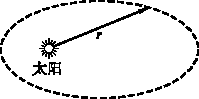
\includegraphics{figure/fig09.02}
  \caption{行星绕太阳的运动}
  \label{fig:09.02}
\end{wrapfigure}
即行星的角动量是守恒的。行星的动
量是不守恒的,因为动量守恒要求没
有外力,而角动量守恒是要求没有外
力矩。在这里所讨论的情况下,有力
而无力矩。我们可以说,不仅引力,
对于任何有心力的作用,若取力心为坐标原点,则质点的角动量
是不变的。

\example 某人造卫星在近地点的速度为$ v _ { 1 } = 8 \text{千米}/\text{秒}$(速度
方向垂直于矢径),近地点离地面高为$ h _ { 1 } = 320 \text{公里} $,远地点离地
面高为$ h _ { 2 } = 1397 \text{公里} $。已知地球的半径为$ R _ { E } = 6378 \text{公里} $。求在远
地点时卫星的速度。

\solution 卫星受地球作用的万有引力是有心力,故对力心力矩为
零,卫星运动时对地球中心的角动量守恒,即
\begin{equation*}
  \vec{l} = \vec{r} \times \vec{P} = \vec{r} \times m \vec{v} =  \text{常量}
\end{equation*}
在近地点及远地点时,$ \vec{r} \perp \vec{v} $(图9 \cdot 3)  ,故由角动量守恒得

\begin{wrapfigure}[5]{r}{14em}
  \centering
  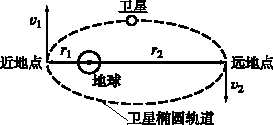
\includegraphics{figure/fig09.03}
  \caption{}
  \label{fig:09.03}
\end{wrapfigure}
\mbox{}\vspace{-1em}\begin{equation*}
  \begin{split}
    l &= m r _ { 1 } v _ { 1 }  \\
    &= m r _ { 2 } v _ { 2 }
  \end{split}
\end{equation*}
所以\vspace{-1.56em}
\begin{equation*}
  v _ { 2 } = \frac { r _ { 1 } } { r _ { 2 } } v _ { 2 }
\end{equation*}
代入已知条件,
\begin{equation*}
  \begin{split}
    r _ { 1 } &= h _ { 1 } + R _ { E } \\
    r _ { 2 } &= h _ { 2 } + R _ { E }
  \end{split}
\end{equation*}
得\vspace{-1.56em}
\begin{equation*}
  \begin{split}
    v _ { 2 } &= \left( \frac { h _ { 1 } + R _ { E } } { h _ { 2 } + R _ { E } } \right) v _ { 1 } \\
    &= 6 . 8 9 \text{公里}/\text{秒}
  \end{split}
\end{equation*}

由角动量守恒,我们可以推知行星运动的性质:

(1)行星轨道处在一确定的平面上,是一条平面曲线。

因为$ \vec{l} = \vec{r} \times m \vec{v} $,所以始终垂直于$ \vec{r} $及$ \vec{v} $所决定的平面(这里
% 259.jpg
$ \vec{r} $与$ \vec{v} $既不平行也不反平行,故总可决定一个平面)。如果行星不
在一固定平面内运动,当它要离开此平面时,速度的方向必不在
此平面内,因此$\vec{l}$的方向发生变化,与角动量守恒相矛盾。故行
\begin{wrapfigure}[6]{r}{13em}
  \centering
  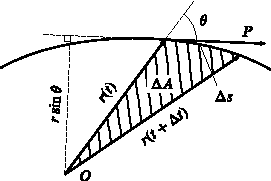
\includegraphics{figure/fig09.04}
  \caption{}
  \label{fig:09.04}
\end{wrapfigure}
星必定始终在同一平面上运
动。

(2)单位时间内扫过的
面积为常量,即所谓面积速
度不变。

根据定义,角动量的大
小为
\begin{equation*}
  \begin{split}
    l &= | \vec{r} \times \vec{P} |  \\
    &= r P \sin \theta  \\
    &= r m v \sin \theta
  \end{split}
\end{equation*}
其中$\theta$是$ \vec{r} $与$ \vec{v} $的夹角。再注意$ v = \dfrac { \Delta s } { \Delta t } $,其中$ \Delta s $是在$ \Delta t $时间
内行星走过的弧长(图94)。则上式成为
\begin{equation*}
  l = m \frac { \Delta s \cdot r \sin \theta } { \Delta t }
\end{equation*}
由图\ref{fig:09.04}知,
\begin{equation*}
  \Delta s \cdot r \sin \theta \approx 2 \Delta A
\end{equation*}
其中$ \Delta A $是行星在$ \Delta t $时间内扫过的面积。所以
\begin{equation*}
  l \approx 2 m \frac { \Delta A } { \Delta t }
\end{equation*}
取$ \Delta t \to 0 $的极限,得
\begin{equation*}
  \begin{split}
    l &= 2 m \frac { \dif A } { \dif t } \\
    &= \text{不变量}
  \end{split}
\end{equation*}
式中$ \dfrac { \dif A } { \dif t } $是行星单位时间内扫过的面积,称为面积速
度。由上式
% 260.jpg
可得

\begin{equation}\label{eqn:09.02.05}
  \frac { \dif A } { \dif t } = \frac { l } { 2m } = \text{不变量}
\end{equation}

\noindent 这就证明了面积速度不变。这也就是开普勒第二定律(见第四
章)。

由开普勒第一定律知行星轨道是个椭圆,如图\ref{fig:09.05}所示。这
\begin{wrapfigure}[7]{r}{17em}
  \centering
  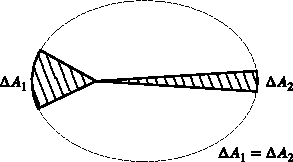
\includegraphics{figure/fig09.05}
  \caption{行星的椭圆轨道}
  \label{fig:09.05}
\end{wrapfigure}样,为了保持面积速度
不变,行星在离太阳近时必定比离太阳远时运
动得快一些。按照地球的轨道,在北半球,冬
季地球处在近日点附近,夏季地球处在远日
点附近。所以,地球绕太阳的公转,在冬季较快而夏季较慢。

在牛顿提出万有引力时,有人就提出一个问题:既然宇宙间
只有引力,为什么宇宙中的物体竟不会塌缩到一块,而物体却还
能处在相当分散的状态?历史上有许多人从不同角度回答过这个
问题。例如,有的人从哲学观点断言:有引力,必定有斥力,所
以不会塌缩,康德就是这种观点。其实这种说法是没有根据的。
有引力,必定有斥力,这不是一条物理上的原理,哲学也不能代
替物理的研究。有引力而不一定会塌缩,原因之一即在于角动量
守恒。臂如我们以太阳而言,它对行星有引力,为什么行星不
会掉到太阳上去呢?原因就是角动量守恒。因为,当物体掉到太
阳上时,不管速度如何,其角动量相对于太阳来说都是零。所
以,只要在太阳系形成时,具有一定的角动量,则整个太阳系就
不可能塌缩到一块去。在距太阳极远的许许多多运动着的物体
中,只有运动方向正对着太阳的那些物体的角动量才为零,而其
他物体的角动量都不是零,这些物体在太阳的万有引力作用下永
% 261.jpg
远不会掉到太阳上去。可见,正是因为太阳与物体之间的作用是
万有引力,它是有心力,才使绝大多数物体不可能掉到太阳上
去,而不需什么其他的斥力。明确指出这一点的是法国的物理学
家拉普拉斯。

对于地球,也有类似的情况。我们知道,地球有时要通过流
星带,但绝不会有很多物体轰击到地球上来,因为地球对它们的
作用是引力,角动量守恒成立,只有极少数开始相对于地球的角
动量为零的那些流星才会掉到地球上来。

人造地球卫星运行一段时间后,会掉回地球上来。这不是由
于地球引力作用,主要是由于大气的摩擦。大气摩擦力总是与卫
星运动方向相反,对地心的力矩不为零,在此力矩作用下,卫星
的角动量逐渐减小,最后掉回地球。我们经常看到陨石掉到地球
上来,原因也是摩擦,由于它在宇宙空间中运行时受到微弱摩擦
作用,使原来角动量从不为零变到零,从而能落到地球上来。
\begin{figurex}
  \centering
  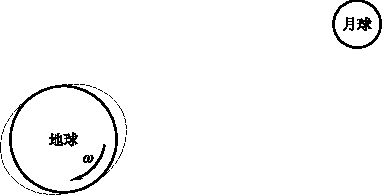
\includegraphics{figure/fig09.06}
  \caption{潮汐}
  \label{fig:09.06}
\end{figurex}

现在我们再讨论一下潮汐现象。在某一海滨,海水的高度每
天都有规律地升降,这就是潮汐现象。潮汐主要是由月球的引力
引起的。在月球引力作用下,地球表面的海水形成如图9.6所示
的形状,在最靠近月球的一侧和最远离月球的一侧凸出来。地球
每天自转一周,因此,地球上确定位置的观察者每天看到两次涨
潮,两次退潮。月球一月绕地球一周,因此,海面凸出部位一月
% 262.jpg
绕地心一周,而地球每天自转一周,所以地球与海面凸出部分之
间有相对运动。两部分之间存在摩擦,其力矩是使地球自转变
慢。现代地学已证明了地球自转的变慢,在3亿年前,地球的一
年是398天,现在的一年是$ 3 6 5  \dfrac { 1 } { 4 } $天,可见变慢不少。到最后,地
球自转速度将与月球绕地球转的角速度相同,也就是说,一个月
转一周,一天将等于一个月。

如果我们把体系扩大些,把地球和月球近似看作一个孤立体
系,它的总角动量应当是守恒的。地、月体系的总角动量等于地球
角动量与月球角动量之和。由于总角动量守恒,所以地球角动量减
少,必定意味着月球角动量增加。根据开普勒定律,月球速度与地
月距离有确定的关系,要想增加角动量,只能增大地、月之间的距
离。也就是说,随着地球自转变慢,月亮将离我们越来越远。
